A raised crosswalk (\figref{xwalk}) is a designated street crossing that simulatneously acts as a speed hump by bringing the level of the roadway to that of the sidewalk.

\begin{figure}
	\centering
	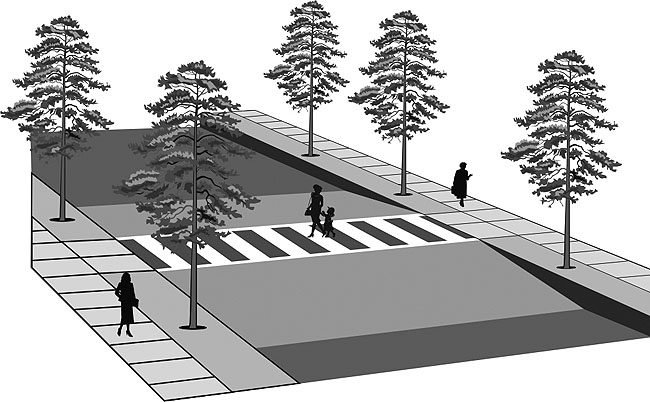
\includegraphics[width=0.7\textwidth]{xwalk.jpg}
	\caption{A raised crosswalk\cite{kimley-xwalk}}\label{fig:xwalk}
\end{figure}

The advantages of such a traffic calming measure include:\begin{itemize}
	\item Forces traffic to slow down, improving pedestrian safety.
	\item Draws attention to the pedestrian, especially when combined with signage and markings.
	\item Makes crossing the street easier for those on wheelchairs.
\end{itemize}

The drawbacks are:\begin{itemize}
	\item The textured materials used tend to be expensive.
	\item Not suitable for emergency or bus routes.
	\item Drainage, especially in snowy or rainy areas, requires additional management.
\end{itemize}

% Please remember to add \use{multirow} to your document preamble in order to suppor multirow cells
% Booktabs require to add \usepackage{booktabs} to your document preamble
\begin{table}[h]
\begin{tabular}{@{}lrrr@{}}
\toprule
\multirow{2}{*}{City and Measure}    & \multicolumn{2}{l}{50th percentile speed (km/h)} & \multirow{2}{*}{Speed reduction (km/hr)} \\ \cmidrule(lr){2-3}
      & Treatment Site           & Control Site          &                  \\ \midrule
\begin{tabular}[l]{@{}l@{}}Durham, NC – Research Drive\\ \textit{Raised crosswalk}\end{tabular}                    & 33.3                     & 39.8                  & 6.5                                      \\
\begin{tabular}[l]{@{}l@{}}Durham, NC – Towerview Drive\\ \textit{Raised crosswalk, overhead flasher}\end{tabular} & 18.5                     & 38.4                  & 19.3                                     \\
\begin{tabular}[l]{@{}l@{}}Montgomery County, MD\\ \textit{Raised Crosswalk}\end{tabular}                          & 34.6                     & 38.6                  & 4.0                                   
\\ \bottomrule
\end{tabular}
\caption{Speed reduction due to raised crosswalks}
\end{table}